%\documentclass[11pt,openright,twoside,letterpaper,onecolumn]{report} %% USE THIS FOR DOUBLE SIDED
\documentclass[11pt,openright,oneside,letterpaper,onecolumn]{report}  %% USE THIS FOR SINGLE SIDED
\newcommand{\thesistitle}{New Methods in Sampling in Molecular Mechanics Simulations and and Improved Algorithm for Calculating Energy Contribution of Implicit Solvent Models}
\newcommand{\thesisauthor}{Joseph Bylund}
\newcommand{\thesisyear}{2013}

%%%
%%% Packages
%%%
\usepackage[dvips]{epsfig}
\usepackage{amsmath}
\usepackage{named}
\usepackage{fancyhdr}
\usepackage{afterpage}

%
% We use the hyperref package and customize it for optimal PDF 
%
%\usepackage[dvipdfm,pdftitle={\thesistitle},pdfauthor={\thesisauthor},pdfpagemode={UseOutlines},letterpaper,bookmarks,bookmarksopen=true,pdfstartview={FitH},bookmarksnumbered=true,]{hyperref}

%%%
%%% Margins
%%%
\paperwidth=8.5in
\paperheight=11in

% 1in + hoffset + oddsidemargin + textwidth + marginparsep + marginparwidth
% For PhD at Columbia we have single side theses and 1.5in left margin
% The settings below leave 1.5 inch margin at the left and 1 inch at the right 
% for US Letter paper
\setlength{\hoffset}{0.0in}
\setlength{\oddsidemargin}{.5in}
\setlength{\textwidth}{6in}
\setlength{\evensidemargin}{0mm}

% 1in + voffset + topmargin + headheight + headsep + textheight + footskip 
% For PhD thesis we also need an extra inch at the bottom
% 1inch = 72 pt
\setlength{\voffset}{0.0in}
\setlength{\topmargin}{.0in}
\setlength{\headheight}{14pt}
\setlength{\headsep}{22pt}
\setlength{\textheight}{8.5in}
\setlength{\footskip}{0pt}

%%%
%%% Spacing
%%%
\newcommand{\singlespace}{\renewcommand{\baselinestretch}{1.15} \small \normalsize}
\newcommand{\oneandhalfspace}{\renewcommand{\baselinestretch}{1.3} \small \normalsize}
\newcommand{\doublespace}{\renewcommand{\baselinestretch}{1.5} \small \normalsize}
\newcommand{\normalspace}{\doublespace}
\footnotesep=1\baselineskip

%%%
%%% Counters depth
%%%
\setcounter{secnumdepth}{3}
\setcounter{tocdepth}{3}

%%%
%%% Title page.
%%%
\newcommand{\thesistitlepage}{
    \normalspace
    \thispagestyle{empty}
    \begin{center}
        \textbf{\LARGE \thesistitle} \\[1cm]
        \textbf{\LARGE \thesisauthor} \\[8cm]
        Submitted in partial fulfillment of the \\
        requirements for the degree \\
        of Doctor of Philosophy \\
        in the Graduate School of Arts and Sciences \\[4cm]
        \textbf{\Large COLUMBIA UNIVERSITY} \\[5mm]
        \thesisyear
    \end{center}
    \clearpage
}

%%%
%%% Copyright page.
%%%
\newcommand{\thesiscopyrightpage}{
    \thispagestyle{empty}
    \strut \vfill
    \begin{center}
      \copyright \thesisyear \\
      \thesisauthor \\
      All Rights Reserved
    \end{center}
    \cleardoublepage
}

%%%
%%% Abstract page.
%%%
\newcommand{\thesisabstract}{
    \thispagestyle{empty}
    \begin{center}
    \textbf{\LARGE ABSTRACT} \\[1cm]
     \textbf{\LARGE \thesistitle} \\[1cm]
     \textbf{\LARGE \thesisauthor} \\[1cm]
    \end{center}
    % abstract should be roughly two pages
The process of bringing drugs to market continues to be a slow and expensive affair.
And despite recent advances in technology, the cost both in monetary terms and in terms of time between target identification and arrival of a new drug on the market continues to increase.

High throughput screening is a first step towards testing a large number of possible bioactive compounds very quickly.
However, the space of possible small molecules is limitless, and high throughput screening is limited both by the size of available libraries and the cost of running such a large number of experiments.
Therefore, advancements in computational drug screening are necessary in order to maining the current rate of progress in modern medicine.

Computational drug design, or computer assisted drug design, offers a possible way of addressing some of the shortfalls of conventional high throughput screening.
Using computational methods, it is possible to estimate parameters such as binding affinity of any small molecule, even those not currently present in any small molecule library, without having to first invest in the often slow and expensive process of finding a synthetic pathway.
Computational methods can be used to screen similar molecules, or mutations in small molecule space, seeking to increase binding affinity to the protein target, and thereby efficacy, while simultaneously minimizing binding affinity to other proteins, decreasing cross reactivity, and reducing toxicity and harmful side effects.

Computational biology methods of drug research can be broadly classified in a number of different ways.
However, one of the most common classifications is according to the methods used to identify possible drug compounds and later optimize those leads.
The first broad category is informatics or artificial intelligence based approaches.
In these approaches, artificial intelligence methods such as neural networks, support vector machines, and qualitative structure-activity relationships (QSAR) are used to identify chemical or structural properties that contribute heavily to binding affinity.
The next category, ligand based approaches, is very useful when there are a large number of known binders for a specific family of proteins.
In this approach, the ligands are clustered using a metric of chemical similarity and new compounds which occupy a similar chemical space are likely to also bind strongly with the protein of interest.
The final class of methods of computational drug design, and the method explored in this thesis, is the diverse class known as structural methods.
These approaches in the most general sense make use of a sampling method to sample a number of protein, or protein-small-molecule interaction conformations and an energy model or scoring function to measure dimensions which would be very difficult and or expensive to measure experimentally.

In this thesis, a number of different sampling methods that are applicable to different questions in computational biology are presented.
Additionally, an improved algorithm for evaluating implicit solvent effects is presented, and a number of improvements in performance, reliability and utility of the molecular mechanics program used are discussed.

    \cleardoublepage
}

%%%
%%% Miscellaneous
%%%
\newcommand{\draft}{
    \renewcommand{\normalspace}{\singlespace}
    \normalspace
    \chapter*{Draft. Version \today}
\clearpage }

\begin{document}
\pagestyle{empty}
\thesistitlepage
\thesiscopyrightpage
\thesisabstract
\pagenumbering{roman}
\pagestyle{plain}
\setlength{\footskip}{0.5in}
\setcounter{tocdepth}{2}
\renewcommand{\contentsname}{Table of Contents}
\tableofcontents
%\cleardoublepage
%\listoffigures
%\cleardoublepage
%\listoftables 
%\cleardoublepage

%%%% Acknowledgments
%~\\[1in] % hack to put space at top.
\textbf{\Huge Acknowledgments}\\

\noindent 
The acknowledgments go here.
The acknowledgments go here.
The acknowledgments go here.
The acknowledgments go here.
The acknowledgments go here.
The acknowledgments go here.
The acknowledgments go here.

%\cleardoublepage


%%%% Dedication page
%\thispagestyle{plain}
%\strut \vfill
%\centerline{\LARGE 
%Dedication text
%}
%\vfill \strut
%\cleardoublepage

%\draft   % Generates a draft version in single-space
%%% BODY
\pagestyle{headings}
\pagenumbering{arabic}

% In the "arabic" section of the thesis, we do not have numbers at  the
% bottom and we want to use the full length of the page to avoid vbox
% underfulls. We use the fancyheaders package to adapt the headers
% according to the  Columbia requirements.
\setlength{\textheight}{8.5in}
\setlength{\footskip}{0in}

% We change the pagestyle 
\fancypagestyle{plain} {%
\fancyhf{}
\fancyhead[LE,RO]{\thepage}
\fancyhead[RE,LO]{\itshape \leftmark}
\renewcommand{\headrulewidth}{0pt}
}
\pagestyle{plain}

\chapter{Introduction}
\label{chapter:intro}

\section{Drug Development}
\label{section:drug_development}

\subsection{Costs of Drug Development}
\label{subsection:costs_of_drug_development}
\subsection{Costs of Drug Development}
\label{subsection:costs_of_drug_development}
\subsection{Costs of Drug Development}
\label{subsection:costs_of_drug_development}
\input{1_intro/drug_development/costs}

\subsection{Computer Assisted Drug Design}
\label{subsection:computer_assisted_drug_design}
\input{1_intro/drug_development/computer_assisted_drug_design}


\subsection{Computer Assisted Drug Design}
\label{subsection:computer_assisted_drug_design}
The ultimate goal of computer assisted drug design is to improve rational drug design by exploiting the continuously increasing processing power available both in high performance super computers, but also in single workstations.
Seeking to supplement the ability of a researcher either by allowing examination of a large number of possible interactions quickly or providing some insight that might be much more difficult to obtain through biochemical experiments, both in terms of time and expense.
Different classes of programs have been developed to help solve each of the distinct steps in the pre-clinical stages of drug development, namely:
\begin{enumerate}
\item Hit Identification – the process of screening a large small molecule database (up to one million or more small molecules) database to identify small molecules which bind a given target protein, or hits.
These hits are usually small molecules with a target binding affinity on the order of micromolar.
\item Hit to lead optimization - the process of modifying these ``hit'' molecules either by substitution or addition of chemical moieties or mixing and matching substructures between given hits, to produce compounds with higher binding affinities than the initial hit compounds.
Hit to lead optimization seeks to improve the micromolar binding affinity of hit compounds to nanomolar affinity or better.
\item Lead Optimization – the final step of modifying lead compounds to increase ``druglikeness'' to ensure that the molecule is sufficiently soluble, well tolerated, and does not disrupt regular cellular function.
\end{enumerate}

\subsubsection{Hit Identification}
\label{subsubsection:hit_identification}
% hit identification in general
The earliest form of hit identification experiments were animal screens, where mutant animals were studied to find the specific gene or protein causing a specific phenotype.
This type of experiment relies on careful genetic controls and breeding, but also some element of luck in observing a relevant phenotype in the first place.
``Brute force'' animal screens have since been improved with extensive mutation libraries and exhaustive non-lethal mutation libraries for organisms such as yeast and {\it Escherichia coli}.
Even so, these screens are slow, often taking three years or longer, and error prone, as performing a large number of repetitive experiments causes even the most fastidious of scientists to lose focus.
High-throughput screening seeks to supplement the human factor with robots, which are capable of performing similar experiments with greater speed and fewer errors.
With the help of this automation it is possible to test the interactions of as many as 100 million different reactions per day \cite{agresti2010ultrahigh}.
Though the high initial cost of high-throughput screening equipment as well as the cost of the small molecule libraries necessary for screening are often prohibitive even to large research institutions.
In order to make this sort of experiment available to a larger number of institutions some research institutions have instituted means of sharing this equipment, through high-throughput screening as a service type arrangements \cite{htsrc,mssr}.

% computational equivalents of hit identification
The direct computational equivalent to high-throughput screening is virtual screening, where a library of small molecules is computational ``docked'' into the active site of the target protein, and some scoring metric is used to identify possible binders.
In this sort of computational screen, he problem of the cost of small molecule libraries is essentially a solved problem in virtual screening as there are readily available libraries of drug-like small molecules for use in virtual screening programs.
For example, the ZINC database provides a library of over seven-hundred thousand commercially available small molecules in a number of different file formats for use in virtual screening \cite{irwin2005zinc}.
Another possibility for hit identification {\it in silico} is through fragment assembly methods.

% early docking history
The first published study using computational docking was published in 1982 by Irwin Kuntz describing a program which would later go on to become the well known DOCK program \cite{kuntz1982geometric}.
Generally docking consists of a method of quickly screening possible protein-small-molecule interaction conformations.
An emphasis is placed on the computational cost of evaluating the energy function over accuracy, as the poses generated by this step are usually fed into structural refinement programs for further sampling and more accurate estimation of energies.
For example in the original Kuntz study, the system only only had six degrees of freedom on which to sample, three translational and three rotational degrees of freedom for the ligand with the protein held fixed.
Along with a hard sphere collision model this provided a sufficiently selective screen to identify the native binding geometry of the heme group to myoglobin as well as thyroid hormone analogs to prealbumin \cite{kuntz1982geometric}.

% growth of pdb data
The rate at which new structures are being deposited into the Protein Data Bank is increasing on an annual basis.
But tools are necessary to draw meaningful insights from this data, hopefully leading to new drugs.
\begin{figure}[H]
\begin{center}
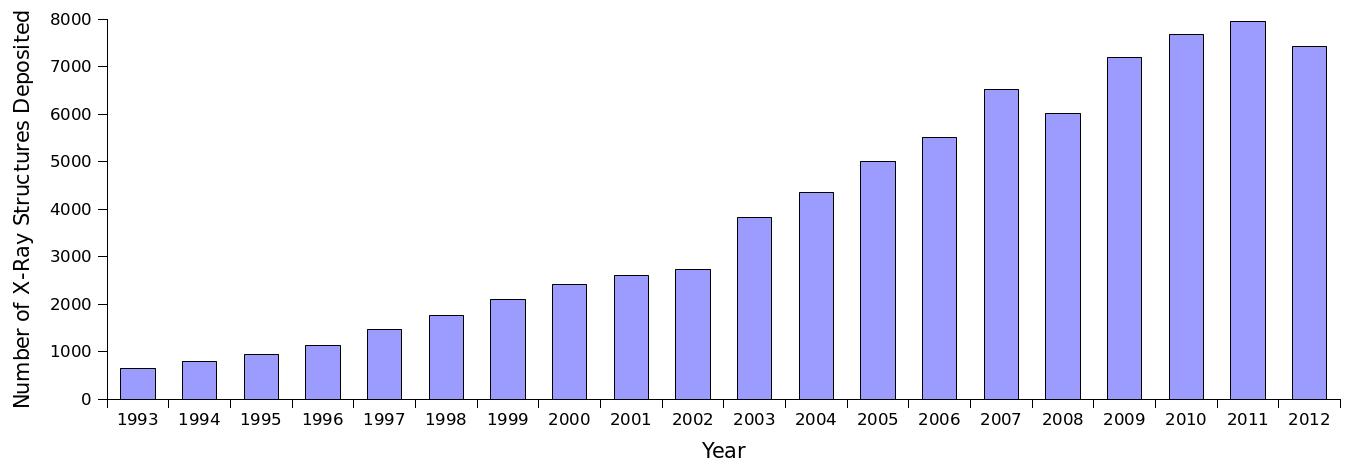
\includegraphics[width=\textwidth]{figures/pdb_deposit_rate.png}
\caption{The rate at which new structures is deposited into the PDB over the last two decades.
Due to a variety of improvements in the field of crystallography this rate has been steadily increasing.}
\label{figure:pdb_growth}
\end{center}
\end{figure}

% expected future growth of pdb
For example a recent increase in the field of crystallography, is ``crystal-less'' crystallography in which small molecules are bound by a porous scaffold matrix.
The regular structure of the matrix imparts a regular packing arrangement, necessary for interpreting diffraction patterns, onto the arrangement of small molecules.
This has the potential to address one of the largest difficulties in obtaining quality structural data for proteins, which is that it is very difficult to purify and crystallize certain proteins \cite{inokuma2013x}.

% unsorted
The number of target molecules of the set of all drugs currently available on the market consists of only about 500 proteins.
The bottleneck in introduction of new chemical entities is not virtual screening, but rather optimizing these hits into higher affinity leads and eventually balancing the requirements across all characteristics to produce a new drug \cite{bleicher2003hit}.

% unsorted
Of the total proteome only ~30,000 are regulated by small molecule binding, making them reasonable targets of drug action.
A large number of these possible drug targets are not implicated in any disease, due to this and a number of other factors, estimates of the total number of these proteins which are possible drug targets is much lower.
Frequently cited numbers for the number of possible drug targets in humans are six-hundred to fifteen-hundred, still significantly higher than the total number of targets which are exploited by current drugs.
The different families of cellular proteins are not equally likely to be targets of drugs.
As of {\the\year} 47\% of current drug targets are enzymes, followed by 30\% being GPCR's \cite{hopkins2002druggable}.

% drug-likeness
The consists of a number of characteristics which are generally true of drug like molecules:
\begin{enumerate}
\item Five or fewer hydrogen bond donors,
\item 500 Da or less total molecular mass
\item high liphophilicity
\item sum of nitrogen and oxygen atoms is not greater than 10 \cite{rule_of_five}
\end{enumerate}

% unedited
Through understanding the protein-ligand conformation and specific contacts they were able to modify a known substrate 
There is an advantage to flexible substrates, which is that they can flex in order to create better contacts with the protein structure increasing binding affinity.
This is especially important as the location of heavy atoms in the target protein is frequently only known to an accuracy of ~0.4 angstroms.
Further specific knowledge of the binding geometry between the initial lead compound and the target makes it possible to computationally screen possible chemical group substituents, to maximize binding affinity, increase solubility or bioavailability.
One of the earliest examples of the successful application of structure based drug design is the carbonic anhydrase inhibitor dorzolamide, in which most of these ideas were applied to find a drug with very high binding affinity \cite{greer1994application}.

% limitations
Despite advantages in speed and cost due to limitations in accuracy computational screening has struggled to produce the same results as empirical screening.
However, more recently virtual screening has succeeded in producing hit rates greater than those from empirical screening techniques.
Virtual screening has been used to identified leads which were later developed into the human immunodeficiency virus (HIV) protease inhibitor Viracept, and the anti-influenza drug Relenza.
\begin{figure}[h]
    \centering
    \begin{subfigure}[b]{0.3\textwidth}
        \centering
        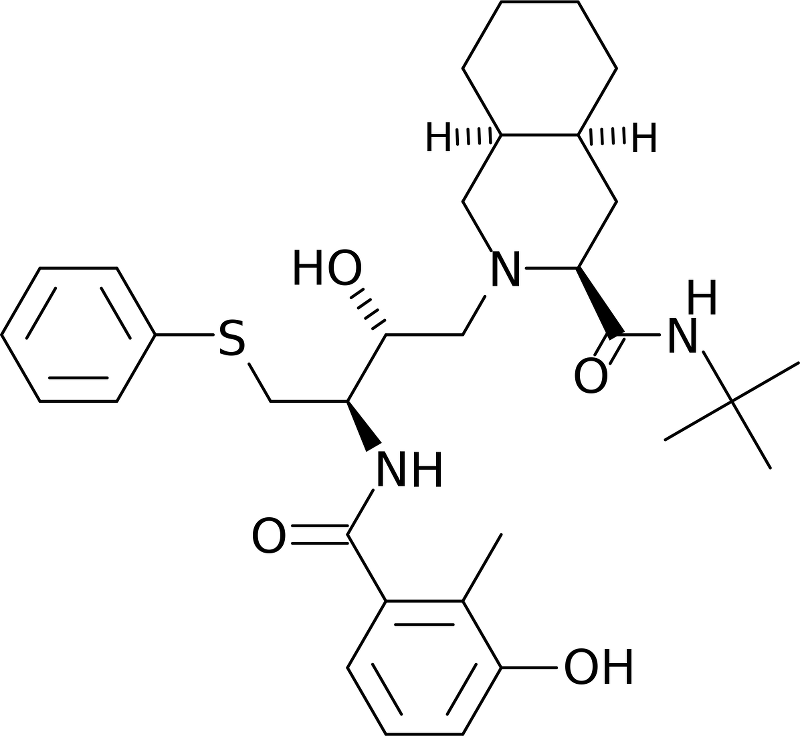
\includegraphics[width=\textwidth]{figures/nelfinavir_small.png}
        \label{fig:nelfinavir_chemical}
        \caption{}
    \end{subfigure}%
    \hspace{0.1\textwidth}
    \begin{subfigure}[b]{0.3\textwidth}
        \centering
        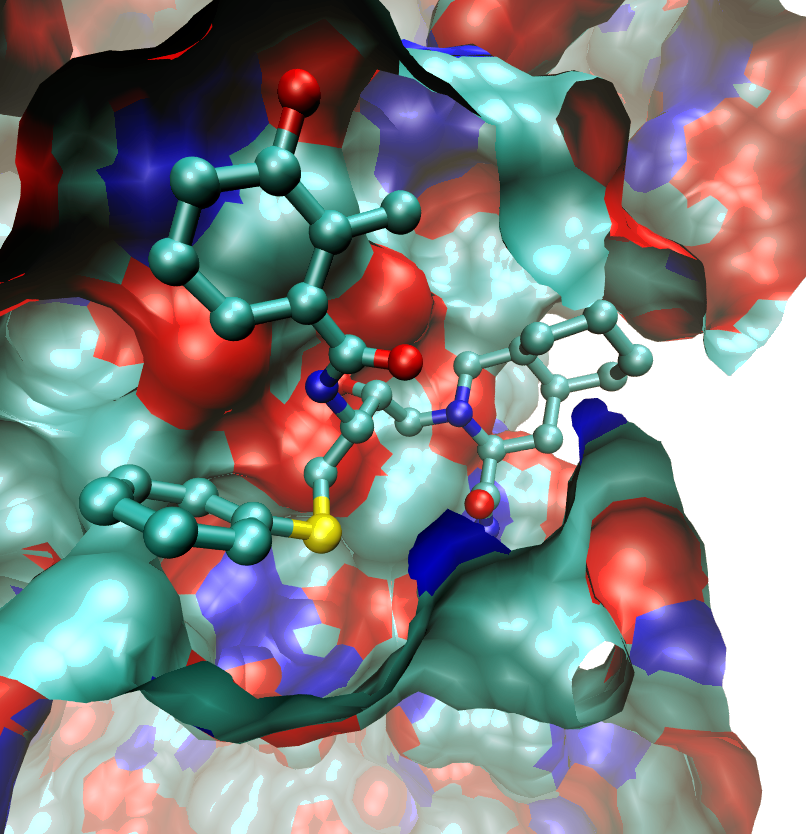
\includegraphics[width=\textwidth]{figures/complexed_nelfinavir_white.png}
        \label{fig:nelfinavir_docked}
        \caption{}
    \end{subfigure}
    \label{fig:nelfinavir}
    \caption{
The HIV protease inhibitor, nelfinavir, marketed under the name Viracept was originally identified using a computational docking screen.
It has a very high binding affinity for its target protein, 2 nM.
Here it is shown crystallized with multidrug variant (ACT) (V82T/I84V) of HIV-1 protease, PDBID 3EL5.
(b) generated with Visual Molecular Dynamics \protect\cite{humphrey1996vmd} and \protect\cite{povray}.
}
\end{figure}
A number of challenges which limit the utility of docking programs have been identified
\begin{enumerate}
\item The number of possible small molecules is essentially unbounded, however only a very small fraction of these ligands are potentially drug compounds. Limiting sampling to this subspace is a challenging problem.
\item The number of conformations of ligand molecules rises exponentially with the number of internal degrees of freedom of the ligand. Sampling the huge conformational space of the ligand becomes a computationally difficult problem on its own.
\item The difficulty of accurately assessing or comparing the energy of different protein-ligand complexes or conformations\cite{shoichet2004virtual}.
\end{enumerate}

% similarity between hits and leads
It has been found that introduced drugs are often very chemically similar the ``hit'' compounds from which they were derived \cite{proudfoot2002drugs}.
So in order to increase the diversity of drugs and find drugs which are able to treat new diseases, or diseases which have evolved resistance to current drugs it may be necessary to either increase the size of the screened database or increase the possible diversity which might be increase through the hit-to-lead step.

%\cite{kitchen2004docking}

\subsubsection{Hit-to-Lead Optimization}
\label{subsubsection:hit_to_lead}
Hit compounds generally have a binding affinity for the target protein on the order of micromolar binding.
The goals of hit-to-lead optimization are to further increase that affinity with the goal of eventually reaching binding affinities on the order of ~10 nanomolar or better, find other molecules with similar chemical characteristics to increase the size and diversity of the set of lead compounds, and screening hit compounds for any obvious issues.
At this stage for computational screening more accurate energy models are required than for the initial screen \cite{jorgensen2004many,gohlke2002approaches,jorgensen2009efficient}.
Depending on the type of ``hit'' compounds identified in the initial screen, hits are either combined through molecular-growing and evolution techniques, or similar structures to the hit compounds can be sampled either by exploring the local chemical space or ``mutation'' of substituents.
In either case, the potential lead compound is docked or grown in the known binding site.
A scoring function which is hopefully well correlated with the binding energy is then used to rank these possible compounds.
Interestingly it is not necessarily the case that the scoring function is anchored in a physical force field, it is possible to use statistical or artificial intelligence approaches with success, so long as they are able to successfully solve the classification problem of distinguishing strong binders from weak binders.
Docking as a means of converting hit compounds to lead compounds is very similar to docking as a means of hit generation, however in this case the small molecule library is much smaller and is generated to cover chemical space surrounding hit compounds.
Additionally whereas for initial hit generation a coarse grained energy function might have been sufficient to differentiate ligands which bind strongly from those which do not bind at all, to convert these ``hits'' to lead compounds it is necessary to use a more sensitive, and necessarily slower, energy model to accurately rank the binding affinity of different small molecules \cite{jorgensen2004many,gohlke2002approaches}.
These energy models will be discussed briefly in \ref{subsection:energy_functions}.

A popular program for building, or mutating lead compounds is Biochemical and Organic Model Builder (BOMB) \cite{barreiro2007docking}.
BOMB can operated as either a hit identification program or as a hit to lead optimization method.
Working to identify new compounds BOMB starts with a number of different small ``core'' scaffolds and attempts to increase binding affinity by adding or replace substituents with favorable interactions while avoiding steric clashes.
BOMB has been successfully used to evolve a hit compound which showed no inhibition of HIV reverse transcriptase into a potent non-nucleoside RT inhibitor with nanomolar level binding \cite{barreiro2007docking}.

Whereas previously, lead compounds were evaluated almost exclusively on binding affinity to the target protein, more recently more weight is being placed on identifying hit compounds which satisfy other characterisitcs besides binding affinity \cite{bleicher2003hit}.
It is important to begin to consider other characterisitcs of the potential drugs earlier in the pre-clinical process, because later it is difficult to make changes which affect characterisitcs such as solubility without significantly altering the binding affinity of an already highly modified hit compound.
As ``lead'' compounds are rarely very chemically distinct from the hits from which they were derived, and increasing binding affinity is actually sometimes an easier problem than addressing some of the other characteristics in the ``rule of five'' it is reasonable to begin by first trying to optimize hit compounds to satisfy some other criteria and postpone maximizing binding affinity \cite{proudfoot2002drugs}.

\subsubsection{Lead Optimization}
\label{subsubsection:lead_optimization}
In lead optimization the compounds which have been identified by the earlier steps in the process are optimized to drug molecules.
The largest differentiating factor between hit-to-lead optimization and lead optimization is the plausibility of the compound to act as a successful drug molecule.
The goals of lead optimization overlap heavily with those of the hit-to-lead stage.
Although this can include increasing binding affinity to the target even further, usually the focus is on other characteristics including selectivity, ease of synthesis, pharmacokinetic properties and intellectual property concerns \cite{keserHu2006hit}.
Computational modelling can help not only identify hit compounds, and convert those initial hits into leads, but also to help estimate absorption, distribution, metabolism, elimination, toxicology, sometimes referred to as the ADME characteristics \cite{kerns2008drug}.

Computational models for ADME characteristics ususally use regression equations or neural networks to predict these characteristics \cite{jorgensen2004many}.

Up to one half of all drugs which do not survive clinical trials, fail to do so because of lack of efficacy, which is influenced both by binding, but also by the absorption characteristics of the molecule.
The number of drugs which fail to make it through clinical trials due to toxcicity is similarly high, about 40\% \cite{li2001screening}.
Advancing a potential drug to clinical trials represents a very large financial investment, and effective computational screens of lead molecules at this point in the process can reduce the rate of failure in clinical trials, thereby having a very large impact on the final costs of new drugs brought to market.



\subsection{Computer Assisted Drug Design}
\label{subsection:computer_assisted_drug_design}
The ultimate goal of computer assisted drug design is to improve rational drug design by exploiting the continuously increasing processing power available both in high performance super computers, but also in single workstations.
Seeking to supplement the ability of a researcher either by allowing examination of a large number of possible interactions quickly or providing some insight that might be much more difficult to obtain through biochemical experiments, both in terms of time and expense.
Different classes of programs have been developed to help solve each of the distinct steps in the pre-clinical stages of drug development, namely:
\begin{enumerate}
\item Hit Identification – the process of screening a large small molecule database (up to one million or more small molecules) database to identify small molecules which bind a given target protein, or hits.
These hits are usually small molecules with a target binding affinity on the order of micromolar.
\item Hit to lead optimization - the process of modifying these ``hit'' molecules either by substitution or addition of chemical moieties or mixing and matching substructures between given hits, to produce compounds with higher binding affinities than the initial hit compounds.
Hit to lead optimization seeks to improve the micromolar binding affinity of hit compounds to nanomolar affinity or better.
\item Lead Optimization – the final step of modifying lead compounds to increase ``druglikeness'' to ensure that the molecule is sufficiently soluble, well tolerated, and does not disrupt regular cellular function.
\end{enumerate}

\subsubsection{Hit Identification}
\label{subsubsection:hit_identification}
% hit identification in general
The earliest form of hit identification experiments were animal screens, where mutant animals were studied to find the specific gene or protein causing a specific phenotype.
This type of experiment relies on careful genetic controls and breeding, but also some element of luck in observing a relevant phenotype in the first place.
``Brute force'' animal screens have since been improved with extensive mutation libraries and exhaustive non-lethal mutation libraries for organisms such as yeast and {\it Escherichia coli}.
Even so, these screens are slow, often taking three years or longer, and error prone, as performing a large number of repetitive experiments causes even the most fastidious of scientists to lose focus.
High-throughput screening seeks to supplement the human factor with robots, which are capable of performing similar experiments with greater speed and fewer errors.
With the help of this automation it is possible to test the interactions of as many as 100 million different reactions per day \cite{agresti2010ultrahigh}.
Though the high initial cost of high-throughput screening equipment as well as the cost of the small molecule libraries necessary for screening are often prohibitive even to large research institutions.
In order to make this sort of experiment available to a larger number of institutions some research institutions have instituted means of sharing this equipment, through high-throughput screening as a service type arrangements \cite{htsrc,mssr}.

% computational equivalents of hit identification
The direct computational equivalent to high-throughput screening is virtual screening, where a library of small molecules is computational ``docked'' into the active site of the target protein, and some scoring metric is used to identify possible binders.
In this sort of computational screen, he problem of the cost of small molecule libraries is essentially a solved problem in virtual screening as there are readily available libraries of drug-like small molecules for use in virtual screening programs.
For example, the ZINC database provides a library of over seven-hundred thousand commercially available small molecules in a number of different file formats for use in virtual screening \cite{irwin2005zinc}.
Another possibility for hit identification {\it in silico} is through fragment assembly methods.

% early docking history
The first published study using computational docking was published in 1982 by Irwin Kuntz describing a program which would later go on to become the well known DOCK program \cite{kuntz1982geometric}.
Generally docking consists of a method of quickly screening possible protein-small-molecule interaction conformations.
An emphasis is placed on the computational cost of evaluating the energy function over accuracy, as the poses generated by this step are usually fed into structural refinement programs for further sampling and more accurate estimation of energies.
For example in the original Kuntz study, the system only only had six degrees of freedom on which to sample, three translational and three rotational degrees of freedom for the ligand with the protein held fixed.
Along with a hard sphere collision model this provided a sufficiently selective screen to identify the native binding geometry of the heme group to myoglobin as well as thyroid hormone analogs to prealbumin \cite{kuntz1982geometric}.

% growth of pdb data
The rate at which new structures are being deposited into the Protein Data Bank is increasing on an annual basis.
But tools are necessary to draw meaningful insights from this data, hopefully leading to new drugs.
\begin{figure}[H]
\begin{center}
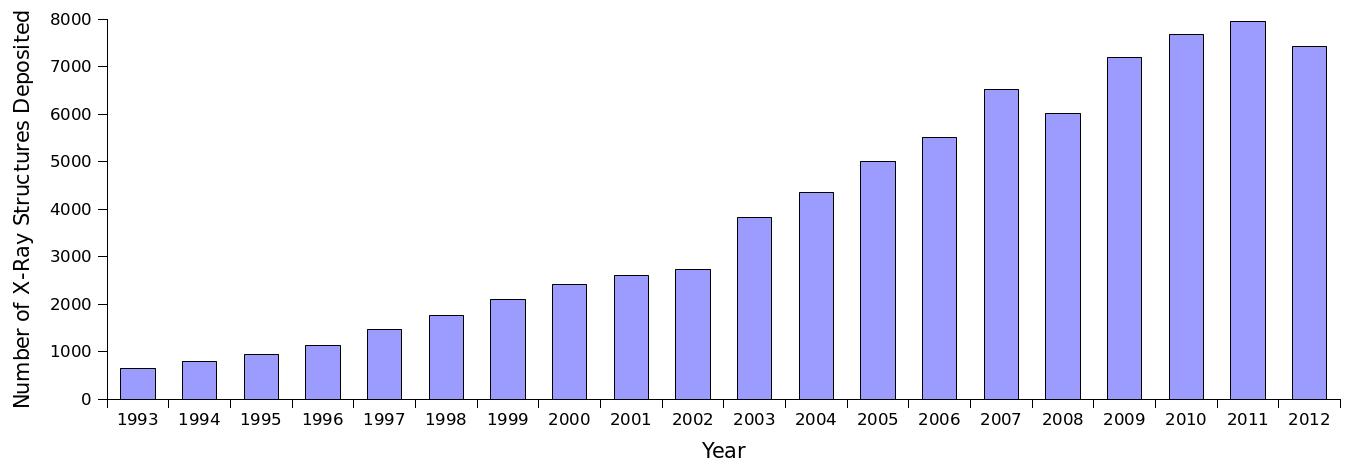
\includegraphics[width=\textwidth]{figures/pdb_deposit_rate.png}
\caption{The rate at which new structures is deposited into the PDB over the last two decades.
Due to a variety of improvements in the field of crystallography this rate has been steadily increasing.}
\label{figure:pdb_growth}
\end{center}
\end{figure}

% expected future growth of pdb
For example a recent increase in the field of crystallography, is ``crystal-less'' crystallography in which small molecules are bound by a porous scaffold matrix.
The regular structure of the matrix imparts a regular packing arrangement, necessary for interpreting diffraction patterns, onto the arrangement of small molecules.
This has the potential to address one of the largest difficulties in obtaining quality structural data for proteins, which is that it is very difficult to purify and crystallize certain proteins \cite{inokuma2013x}.

% unsorted
The number of target molecules of the set of all drugs currently available on the market consists of only about 500 proteins.
The bottleneck in introduction of new chemical entities is not virtual screening, but rather optimizing these hits into higher affinity leads and eventually balancing the requirements across all characteristics to produce a new drug \cite{bleicher2003hit}.

% unsorted
Of the total proteome only ~30,000 are regulated by small molecule binding, making them reasonable targets of drug action.
A large number of these possible drug targets are not implicated in any disease, due to this and a number of other factors, estimates of the total number of these proteins which are possible drug targets is much lower.
Frequently cited numbers for the number of possible drug targets in humans are six-hundred to fifteen-hundred, still significantly higher than the total number of targets which are exploited by current drugs.
The different families of cellular proteins are not equally likely to be targets of drugs.
As of {\the\year} 47\% of current drug targets are enzymes, followed by 30\% being GPCR's \cite{hopkins2002druggable}.

% drug-likeness
The consists of a number of characteristics which are generally true of drug like molecules:
\begin{enumerate}
\item Five or fewer hydrogen bond donors,
\item 500 Da or less total molecular mass
\item high liphophilicity
\item sum of nitrogen and oxygen atoms is not greater than 10 \cite{rule_of_five}
\end{enumerate}

% unedited
Through understanding the protein-ligand conformation and specific contacts they were able to modify a known substrate 
There is an advantage to flexible substrates, which is that they can flex in order to create better contacts with the protein structure increasing binding affinity.
This is especially important as the location of heavy atoms in the target protein is frequently only known to an accuracy of ~0.4 angstroms.
Further specific knowledge of the binding geometry between the initial lead compound and the target makes it possible to computationally screen possible chemical group substituents, to maximize binding affinity, increase solubility or bioavailability.
One of the earliest examples of the successful application of structure based drug design is the carbonic anhydrase inhibitor dorzolamide, in which most of these ideas were applied to find a drug with very high binding affinity \cite{greer1994application}.

% limitations
Despite advantages in speed and cost due to limitations in accuracy computational screening has struggled to produce the same results as empirical screening.
However, more recently virtual screening has succeeded in producing hit rates greater than those from empirical screening techniques.
Virtual screening has been used to identified leads which were later developed into the human immunodeficiency virus (HIV) protease inhibitor Viracept, and the anti-influenza drug Relenza.
\begin{figure}[h]
    \centering
    \begin{subfigure}[b]{0.3\textwidth}
        \centering
        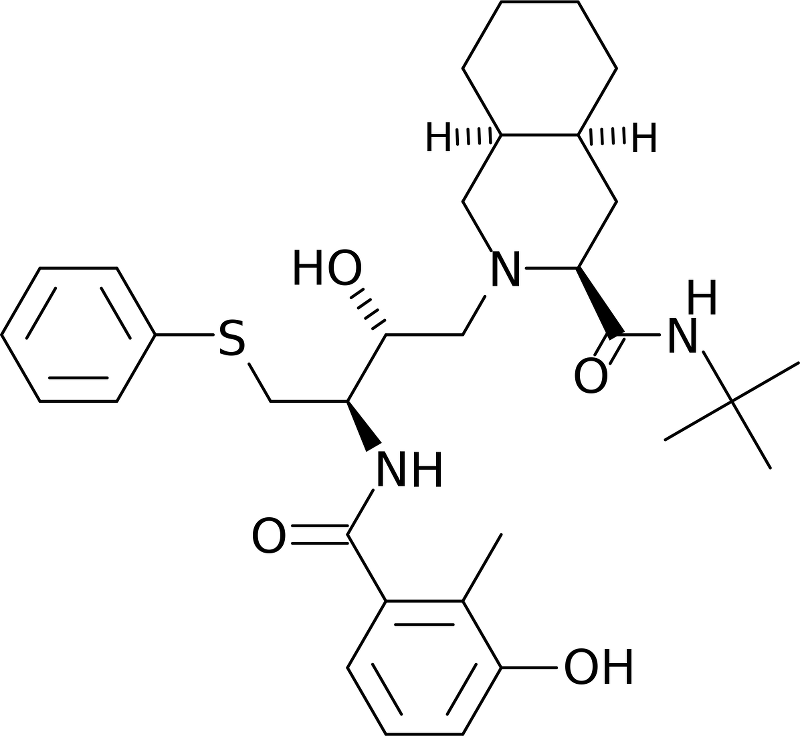
\includegraphics[width=\textwidth]{figures/nelfinavir_small.png}
        \label{fig:nelfinavir_chemical}
        \caption{}
    \end{subfigure}%
    \hspace{0.1\textwidth}
    \begin{subfigure}[b]{0.3\textwidth}
        \centering
        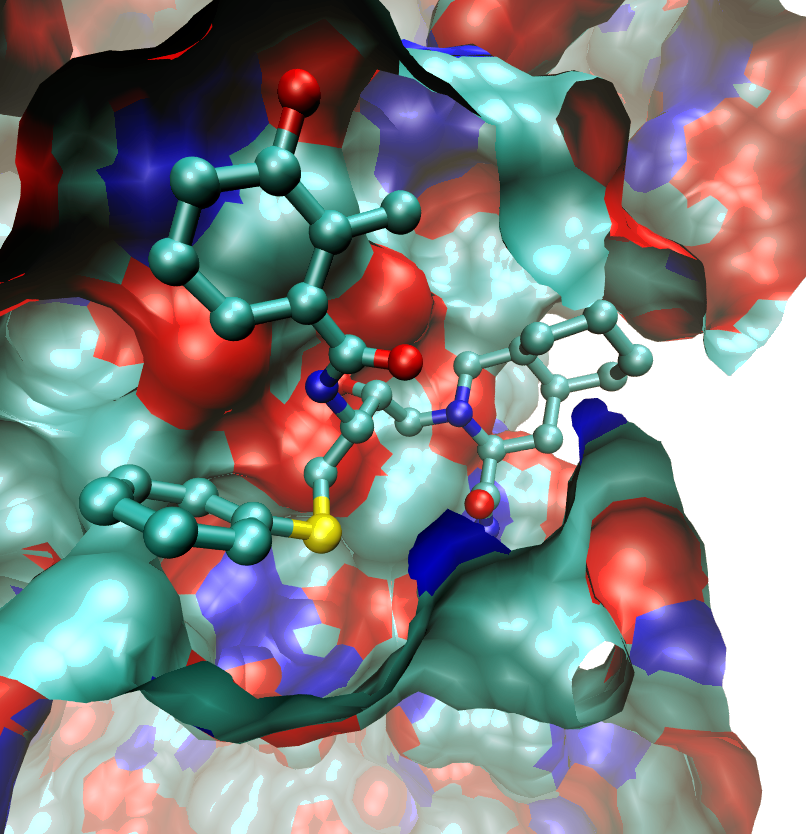
\includegraphics[width=\textwidth]{figures/complexed_nelfinavir_white.png}
        \label{fig:nelfinavir_docked}
        \caption{}
    \end{subfigure}
    \label{fig:nelfinavir}
    \caption{
The HIV protease inhibitor, nelfinavir, marketed under the name Viracept was originally identified using a computational docking screen.
It has a very high binding affinity for its target protein, 2 nM.
Here it is shown crystallized with multidrug variant (ACT) (V82T/I84V) of HIV-1 protease, PDBID 3EL5.
(b) generated with Visual Molecular Dynamics \protect\cite{humphrey1996vmd} and \protect\cite{povray}.
}
\end{figure}
A number of challenges which limit the utility of docking programs have been identified
\begin{enumerate}
\item The number of possible small molecules is essentially unbounded, however only a very small fraction of these ligands are potentially drug compounds. Limiting sampling to this subspace is a challenging problem.
\item The number of conformations of ligand molecules rises exponentially with the number of internal degrees of freedom of the ligand. Sampling the huge conformational space of the ligand becomes a computationally difficult problem on its own.
\item The difficulty of accurately assessing or comparing the energy of different protein-ligand complexes or conformations\cite{shoichet2004virtual}.
\end{enumerate}

% similarity between hits and leads
It has been found that introduced drugs are often very chemically similar the ``hit'' compounds from which they were derived \cite{proudfoot2002drugs}.
So in order to increase the diversity of drugs and find drugs which are able to treat new diseases, or diseases which have evolved resistance to current drugs it may be necessary to either increase the size of the screened database or increase the possible diversity which might be increase through the hit-to-lead step.

%\cite{kitchen2004docking}

\subsubsection{Hit-to-Lead Optimization}
\label{subsubsection:hit_to_lead}
Hit compounds generally have a binding affinity for the target protein on the order of micromolar binding.
The goals of hit-to-lead optimization are to further increase that affinity with the goal of eventually reaching binding affinities on the order of ~10 nanomolar or better, find other molecules with similar chemical characteristics to increase the size and diversity of the set of lead compounds, and screening hit compounds for any obvious issues.
At this stage for computational screening more accurate energy models are required than for the initial screen \cite{jorgensen2004many,gohlke2002approaches,jorgensen2009efficient}.
Depending on the type of ``hit'' compounds identified in the initial screen, hits are either combined through molecular-growing and evolution techniques, or similar structures to the hit compounds can be sampled either by exploring the local chemical space or ``mutation'' of substituents.
In either case, the potential lead compound is docked or grown in the known binding site.
A scoring function which is hopefully well correlated with the binding energy is then used to rank these possible compounds.
Interestingly it is not necessarily the case that the scoring function is anchored in a physical force field, it is possible to use statistical or artificial intelligence approaches with success, so long as they are able to successfully solve the classification problem of distinguishing strong binders from weak binders.
Docking as a means of converting hit compounds to lead compounds is very similar to docking as a means of hit generation, however in this case the small molecule library is much smaller and is generated to cover chemical space surrounding hit compounds.
Additionally whereas for initial hit generation a coarse grained energy function might have been sufficient to differentiate ligands which bind strongly from those which do not bind at all, to convert these ``hits'' to lead compounds it is necessary to use a more sensitive, and necessarily slower, energy model to accurately rank the binding affinity of different small molecules \cite{jorgensen2004many,gohlke2002approaches}.
These energy models will be discussed briefly in \ref{subsection:energy_functions}.

A popular program for building, or mutating lead compounds is Biochemical and Organic Model Builder (BOMB) \cite{barreiro2007docking}.
BOMB can operated as either a hit identification program or as a hit to lead optimization method.
Working to identify new compounds BOMB starts with a number of different small ``core'' scaffolds and attempts to increase binding affinity by adding or replace substituents with favorable interactions while avoiding steric clashes.
BOMB has been successfully used to evolve a hit compound which showed no inhibition of HIV reverse transcriptase into a potent non-nucleoside RT inhibitor with nanomolar level binding \cite{barreiro2007docking}.

Whereas previously, lead compounds were evaluated almost exclusively on binding affinity to the target protein, more recently more weight is being placed on identifying hit compounds which satisfy other characterisitcs besides binding affinity \cite{bleicher2003hit}.
It is important to begin to consider other characterisitcs of the potential drugs earlier in the pre-clinical process, because later it is difficult to make changes which affect characterisitcs such as solubility without significantly altering the binding affinity of an already highly modified hit compound.
As ``lead'' compounds are rarely very chemically distinct from the hits from which they were derived, and increasing binding affinity is actually sometimes an easier problem than addressing some of the other characteristics in the ``rule of five'' it is reasonable to begin by first trying to optimize hit compounds to satisfy some other criteria and postpone maximizing binding affinity \cite{proudfoot2002drugs}.

\subsubsection{Lead Optimization}
\label{subsubsection:lead_optimization}
In lead optimization the compounds which have been identified by the earlier steps in the process are optimized to drug molecules.
The largest differentiating factor between hit-to-lead optimization and lead optimization is the plausibility of the compound to act as a successful drug molecule.
The goals of lead optimization overlap heavily with those of the hit-to-lead stage.
Although this can include increasing binding affinity to the target even further, usually the focus is on other characteristics including selectivity, ease of synthesis, pharmacokinetic properties and intellectual property concerns \cite{keserHu2006hit}.
Computational modelling can help not only identify hit compounds, and convert those initial hits into leads, but also to help estimate absorption, distribution, metabolism, elimination, toxicology, sometimes referred to as the ADME characteristics \cite{kerns2008drug}.

Computational models for ADME characteristics ususally use regression equations or neural networks to predict these characteristics \cite{jorgensen2004many}.

Up to one half of all drugs which do not survive clinical trials, fail to do so because of lack of efficacy, which is influenced both by binding, but also by the absorption characteristics of the molecule.
The number of drugs which fail to make it through clinical trials due to toxcicity is similarly high, about 40\% \cite{li2001screening}.
Advancing a potential drug to clinical trials represents a very large financial investment, and effective computational screens of lead molecules at this point in the process can reduce the rate of failure in clinical trials, thereby having a very large impact on the final costs of new drugs brought to market.


\section{Molecular Modeling}
\label{section:molecular_modeling}
Molecular modeling seeks to gain new insights into the real world behavior of molecules by mimicking these molecules, usually using computer simulations.
According to the theory of ``minimal frustration'' the protein native state is not only a low energy state, but is also stable \cite{bryngelson1987spin}.
So the prediction of native or native-like conformations focuses on finding those conformations which have a low potential energy.
As measuring the true potential energy of a system is very difficult or impossible computational models seek to reproduce the qualitative behavior of the energy surface.
Quantum mechanics calculations are often viewed as the gold standard with respect to intramolecular energy calculations.
However, despite the accuracy of quantum mechanics, its application to large systems such as proteins is currently limited due to the amount of time necessary to perform quantum mechanics calculations on a large number of atoms.
Instead quantum mechanics calculations have been used to parameterize a majority of the most popular molecular mechanics force fields currently in use, including:
\begin{enumerate}
\item AMBER \cite{weiner1984new},
\item OPLS-AA \cite{kaminski1994free},
\item and CHARMM \cite{mackerell2002charmm}.
\end{enumerate}

The earliest molecular mechanics force fields either modeled groups of atoms as a unit, hydrogens being grouped with their bound heavy atom \cite{jorgensen1988opls}, or even each residue as a unit \cite{lee1999energy}, both to reduce the number of parameters in the model and to increase the speed of computations.
Although {\it ab initio} folding experiments are theoretically interesting, they are generally not practical both because of the difficulty in simulating such a large system for the time-frame necessary to observe behaviors like folding, and also because structural models for many proteins are available either directly as X-ray structures, or indirectly through homology.

\begin{figure}[h]
\begin{center}
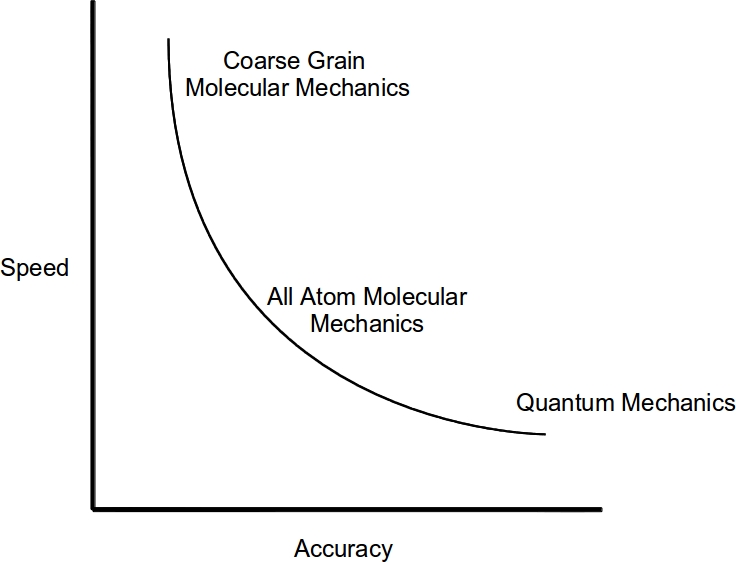
\includegraphics[width=0.7\textwidth]{figures/conservation_of_annoyance.png}
\caption{To an extent it is always possible to either increase accuracy or decrease running time, or the cost of an experiment.
New scientific methods should allow one to increase accuracy while not spending additional time.}
\label{figure:conservation_of_annoyance}
\end{center}
\end{figure}

Because of the evolutionary cost of mis-folded proteins, proteins have been selected to minimize mis-folding, making the general shape of the potential energy surface roughly funnel shaped with the native structure at the minimum \cite{leopold1992protein}.
Despite this shape, the energy landscape of proteins is a very ``jagged'' surface with a large number of local minima \cite{tsai1999folding}.

Even the smallest enzyme contains 62 amino acids, and has thousands of degrees of freedom \cite{chen19924}, and larger enzymes are regularly more than 1000 amino acids.
The number of degrees of freedom of these systems make any attempt to analytically solve for a global minimum energy conformation impossible, and require other methods of generating plausible conformations.
In order to compensate for this a number of different sampling methods have been developed.

%\subsection{Sampling Methods}
%\label{subsection:sampling_methods}

%    \subsubsection{Minimization}
%    \label{subsubsection:minimization}
%    Minimization techniques seek to find the lowest energy conformation in a given potential well.
Generally, they make no attempt to sample outside of that well, and therefore are frequently implemented as a final stage in sampling, in order to relieve any unfavorable interactions in proposed structures.
There are a large number of different minimization techniques, and they will not be covered in any real depth here, please see the original papers for more details, or \cite{schlick2010molecular} for a review.
As the basic terms of the general molecular mechanics potential energy function are differentiable, and discounting for the moment the significant effects of solvent, it is possible to solve for the energy gradient, or force on every atom for a given conformation.
A few minimizations methods include:
\begin{enumerate}
\item ``Steepest descent'', conceptually the simplest minimization algorithm, in which the gradient is calculated at each step, and the size of the step is proportional to the magnitude of the gradient \cite{levitt1969refinement,bixon1967potential}.
\item ``Newton'' methods instead of approximating the gradient as a linear function in a small neighborhood, express the gradient, as a quadratic function.  This has been shown to converge more quickly than steepest descent \cite{ponder1987efficient}.  
Discrete Newton and Quasi-Newton methods use numeric estimation techniques instead of analytically solving for the gradient \cite{schlick2010molecular}.
\item ``Truncated Newton'' methods find an approximate solution to Newton's equations, forcing the residual to approach zero as the series converges \cite{dembo1983truncated}. 
\end{enumerate}

% molecular mechanics burkert allinger

%Quasi-Newton methods like ABNR of CHARMM estimate the hessian, instead of computing it directly, by accumulating residuals over multiple steps \cite{chu2003super}.


%    \subsubsection{Monte-Carlo Sampling}
%    \label{subsubsection:monte_carlo}
%    Metropolis Monte-Carlo simulation was originally developed in the 1950's to provide rapid sampling of the solution space of many variable problems \cite{metropolis1953equation,hastings1970monte}.
Monte-Carlo techniques generate a sequence of states from a distribution by proposing a new state based only on the current state 
If the ensemble average is the same as the sequence average, a Monte Carlo Markov chain can be used to estimate ensemble averages, this is known as {\it ergodicicy} \cite{schlick2010molecular}.
Another requirement is {\it detailed balance} that the probability of transition from a state $X_{i}$ to a state $X_{i+1}$ is the same as the probability of the reverse transition, i.e. $X_{i+1}$ to $X_{i}$.
By setting the probability of acceptance to
\input{equations/metropolis_acceptance}
these conditions are met.

In molecular mechanics, Metropolis Monte Carlo provides a very efficient means of sampling conformation space and a simple method of estimating the distribution of states.
Modifications on this method, such as annealing, where the temperature is continuously decreased over the course of the simulation, or umbrella sampling, which attempts to achieve better sampling in cases where a potential energy barrier divides two or more states from each other \cite{torrie1977nonphysical}.
While Monte Carlo sampling techniques are very fast to provide new states, the majority of these states reflect higher energy conformations.
Since it is of practical biological interest, Monte Carlo minimization has been developed to increase the rate at which minima are sampled \cite{li1987monte}.



%    \subsubsection{Analytic Loop Closure}
%    \label{subsubsection:analytic_loop_closure}
%    Subsequences with regular secondary structures, i.e. $\alpha$-helices and $\beta$-sheets are generally better conserved, and therefore likely to be well covered by simple homology models \cite{kolodny2005inverse,petrey2003using}.
The intervening ``random coil'' or loop regions often play a large role in determining protein specificity for a specific ligand, as in antigen-antibody binding \cite{bajorath1996comparison}, small protein toxins to the receptors they target \cite{wu1996functional}, or transcription factors to specific DNA sequences \cite{jones1999protein}.

Loop closure or prediction is a significant part of homology modeling \cite{petrey2003using} and building structures consistent with X-ray refraction data.
Therefore, in order to accurately predict three dimensional structure through homology models, infer protein binding partners and function, or even build a three dimensional structure consistent with both X-ray data and physical constraints, accurately predicting these loop regions is critical \cite{fiser2000modeling}.

The loop closure question is, given two fixed endpoints and a flexible loop, or actuator, how does one find a loop conformation, or set of conformations, that connects the two endpoints.
Because similar problems are frequently encountered in the field of robotics, a number of loop closure algorithms have been adapted from robotics \cite{kolodny2005inverse}.
The first of these algorithms is analytical loop closure, where a conformation that satisfies the closure criteria is solved for directly by solving a system of equations.
Though this problem can be solved analytically for small loops \cite{wedemeyer1999exact,go1970ring,bruccoleri1985chain,palmer1991standard}, the difficulty of the problem increases as loop length grows and the number of degrees of freedom of the loop section increases.
Additionally, these closure constraints make sampling multiple different conformations more difficult \cite{cortes2005sampling}, though it is possible to hierarchically solve sub-loops in order to generate conformations for possible complete loop conformations \cite{wedemeyer1999exact}.


%    \subsubsection{Random Tweak}
%    \label{subsubsection:tweak}
%    Random tweak, like CCD, is a method of producing and sampling closed loop conformations.
It begins in much the same way as CCD, by randomizing $\phi$ and $\psi$ dihedral angles of the loop backbone.
Random tweak seeks to close the loop while retaining dihedral angles as close to the randomized starting structure as possible.
By adjusting each dihedral only a small amount at a time and staying in the region where $sin(\theta) \approx \theta$, it is possible to formulate a set of linear equations to solve for a set of $\Delta\theta_{i}$, which minimizes the distance between the crystal position of the atom to be closed and the random position.
Because the assumption $sin(\theta) \approx \theta$ only holds for small $\theta$, the maximum change in angle is limited to 10 degrees in the original implementation of the random tweak algorithm.
Because almost all structures predicted using the random tweak or cyclic coordinate descent produce closed loops, a much smaller fraction of time is spent sampling loops that do not satisfy the closure criteria, making these algorithms very efficient \cite{fine1986predicting,shenkin1987predicting}.


%    \subsubsection{Cyclic Coordinate Descent}
%    \label{subsubsection:cyclic_coordinate_descent}
%    Another robotics algorithm which has been successfully applied to protein loop closure is Cyclic Coordinate Descent (CCD) \cite{canutescu2003cyclic}.
As the length of a flexible loop grows the number of degrees of freedom increases and the possible solution space grows exponentially. 
Cyclic coordinate descent seeks to close the loop by adjusting the degrees of freedom, in this case the $\phi$ and $\psi$ dihedral angles, sequentially and possibly iterating over each degree of freedom multiple times until the loop is closed.
This method is able to solve for conformations very quickly, and the likelyhood of closing a loop {\it increases} as the number of degrees of freedom of the system increases.

In cyclic coordinate descent the $\phi$ and $\psi$ angles of each loop backbone residue are first randomized.
Then a loop dihedral is chosen at random, and varied to move the last atom of the loop as near as possible to its desired position.
A new dihedral is chosen and optimized until the loop is closed.
It is possible that this procedure does not converge to a closed state, however experiments have shown that this is very unlikely even for extended loops with few degrees of freedom, $ < 2\%$ failure rate for 4 residue loops.
Solving for the ideal dihedral angle at each step is a simple optimization problem making CCD a very fast algorithm \cite{wang1991combined,canutescu2003cyclic}.
In experiments CCD produces closed loop candidates in ~1/6 the time of the random tweak method.

A variation on cyclic coordinate descent seeks to close the loop by not only requiring atom closure, but by requiring that the entire backbone of the closure residue is superimposed, within some geometric similarity tolerance, between the predicted and crystal structure.
This constrainint ensures that the angles and dihedrals of the closure residue are reasonable\cite{canutescu2003cyclic}.


%    \subsubsection{Rotamer Assembly}
%    \label{subsubsection:rotamer_assembly}
%    Rotamer assembly or systematic search shares some similarity with fragment buildup techniques in that it uses a rotamer library to assemble possible loops.
This rotamer library represents the common backbone dihedrals for each amino acid.
This method operates by dividing the loop into two pieces, usually in half, and considering all possible half loops which can be built using rotamer library \cite{moult1986algorithm}.
For each side of the loop a ``tree'' is considered in both a physical sense, that the hemi-loop branches as it grows away from its anchor, and a decision tree sense, in that every residue represents a decision where a single rotamer is selected from the rotamer library.
When the hemi-trees for each side of the gap are fully constructed some closure criteria is applied, in the case of the original systematic search geometric agreement is required of the entire mid-residue \cite{moult1986algorithm}, however a more lax criteria is applied in the case of the PLOP where only one atom is required to be approximately superimposed \cite{jacobson2004hierarchical}.
By carefully pruning trees during the building process, and biasing the search towards occupied regions of $\phi$-$\psi$ space, systematic search can be quite efficient, spending little time sampling implausible regions of conformation space.
Additionaly, by building residue pairs, using a smaller
 possibly restricting the rotamer library by building multiple residues at a time this sort of procedure has been used to build loops of 20+ residues \cite{zhao2011progress}.


% \cite{kolodny2005inverse}


\subsection{Energy Functions}
\label{subsection:energy_functions}
    \subsubsection{The General Form of the Energy Model}
    \label{subsubsection:energy_general_form}
    Some energy models do not seek to accurately rank potential conformations, fast ``screening'' functions attempt to quickly differentiate physically impossible conformations from plausible conformations without performing an expensive minimization or energy calculation step.
Application of these screening functions has the potential to greatly reduce the number of potential conformations that must be scored using the full detail energy function, greatly decreasing the overall cost of conformation prediction.
These screening criteria can be applied either during the sampling procedure, potentially eliminating sampling of a large area of excluded conformation space, or after sampling before a more expensive energy function is applied to rank conformations.
Effective screening criteria have a large impact on the total performance of a structure prediction method.

One of the earliest screening criteria was the hard sphere overlap collision detection \cite{levinthal1966molecular}, and this method is consistently included in screening scriteria.
Other screens include:
\begin{enumerate}
\item bounds on bond lengths and angles, as a single bond which deviates significantly from equilibrium can dominate the energy of a conformation,
\item limitations on $\phi$-$\psi$ space occuped by backbone dihedrals corresponding to the Ramachandran plot of the residue,
\item limiting side chain dihedrals to staggered conformations, which correspond to the low energy well of side chain dihedral space \cite{moult1986algorithm},
\item excluding structuctures which present excessive solvent accessible surface area, as this conflicts with the hydrophobic effect, which has a large effect on the conformation of the native state \cite{chothia1975principles}
\item limitations on the number of ``dry'' cavities, and the number of internal charged residues \cite{moult1986algorithm}
\end{enumerate}

The general form of most molecular mechanics energy potentials is reasonably consistent, with bonds and angles being modeled as a spring, dihedrals as a Fourier series.
\input{equations/opls.tex}
\input{equations/bonds.tex}
\input{equations/angles.tex}
\input{equations/dihedrals_compact.tex}
The non-bonded terms are modeled as a Columbic potential between any point charges and a Lennard-Jones or 6-12 potential between any non-bonded atoms.
These non-bonded atoms are phased in by a ``fudge factor'' for atoms in a 1-4 configuration.
\input{equations/nonbonded.tex}
Where $\sigma_{ij} = \sqrt{\sigma_{ii} \sigma_{jj}}$ and $\epsilon_{ij} = \sqrt{\epsilon_{ii}\epsilon_{jj}}$ \cite{jorgensen1996development}.



    \subsubsection{Molecular Surfaces}
    \label{subsubsection:molecular_surfaces}
    Central to the discussion of solvent is a discussion of how to formulate the surface of a protein.
The most frequently used formulations of surface area include:
\begin{enumerate}
\item The Van der Waals (VDW) surface is the surface formed by the VDW radius of each molecule, though sometimes differing parameters are used for the VDW radii, and the ideal radii may even vary by application.
\item The solvent accessible surface, which is defined as the surface traced by the center of a spherical probe ``rolled'' over the VDW surface \cite{richards1977areas}.  This idea is very closely related to the idea of the solvent excluded volume, or the shape of the solvent cavity enforced by the VDW surface of the molecule \cite{richmond1984solvent}.
\item The molecular surface, or Connolly surface, is composed of the VDW surface in areas where the spherical probe touches the VDW surface, in union with all points on the probe ``between'' two points on the VDW surface when the probe is contacting multiple atoms \cite{connolly1983analytical}, put another way the surface of the volume which intersects no possible probe location.
\end{enumerate}
Frequently these surfaces are approximated numerically, using the Shrake-Rupley algorithm \cite{shrake1973environment}, by considering a spherical mesh about every atom and including only points which satisfy the definition of the surface, or using these points to interpolate a surface.

The significance of surface area is determined by physical constraints but can be well illustrated by a number of observations about proteins.
First the ratio of total area of a theoretical unfolded, i.e. linearly arranged, protein to its length is almost among proteins, only varying by \textapprox 3\% between different proteins.


\subsection{Solvent Models}
\label{subsubsection:solvent_models}
The section on solvent models.





%%% Bibliography
\part{Bibliography}
\addcontentsline{toc}{chapter}{Bibliography}
\bibliography{refs}
\bibliographystyle{named} 

\end{document}


%Metropolis Monte-Carlo simulation was originally developed in the 1950's to provide rapid sampling of the solution space of many variable problems \cite{metropolis1953equation,hastings1970monte}.
Monte-Carlo techniques generate a sequence of states from a distribution by proposing a new state based only on the current state 
If the ensemble average is the same as the sequence average, a Monte Carlo Markov chain can be used to estimate ensemble averages, this is known as {\it ergodicicy} \cite{schlick2010molecular}.
Another requirement is {\it detailed balance} that the probability of transition from a state $X_{i}$ to a state $X_{i+1}$ is the same as the probability of the reverse transition, i.e. $X_{i+1}$ to $X_{i}$.
By setting the probability of acceptance to
\begin{equation}
\label{equation:metropolis_acceptance}
P(x \rightarrow x') = min\left(1,e^{-\frac{{\Delta}E}{k_{B}T}}\right)
\end{equation}

these conditions are met.

In molecular mechanics, Metropolis Monte Carlo provides a very efficient means of sampling conformation space and a simple method of estimating the distribution of states.
Modifications on this method, such as annealing, where the temperature is continuously decreased over the course of the simulation, or umbrella sampling, which attempts to achieve better sampling in cases where a potential energy barrier divides two or more states from each other \cite{torrie1977nonphysical}.
While Monte Carlo sampling techniques are very fast to provide new states, the majority of these states reflect higher energy conformations.
Since it is of practical biological interest, Monte Carlo minimization has been developed to increase the rate at which minima are sampled \cite{li1987monte}.


%\chapter{Cross Docking}
\label{chapter:cross_docking}
\section{Cross Docking}
\label{section:cross_docking}
\subsection{Cross Docking}
\label{subsection:cross_docking}
\cite{jacobson2004hierarchical}

%\chapter{Computational Mutation Scanning}
\label{chapter:mutations}
\section{Computational Mutation Scanning}
\label{section:mutations}
\subsection{Computational Mutation Scanning}
\label{subsection:mutations}
\cite{jacobson2004hierarchical}

%\chapter{Hash-Based Implicit Solvent}
\label{chapter:cell_solvent}
\section{Hash-Based Implicit Solvent}
\label{section:cell_solvent}
\subsection{Hash-Based Implicit Solvent}
\label{subsection:cell_solvent}
\cite{jacobson2004hierarchical}


%\part{Title for the first part}
%\label{sec:corpus}
%\input{sample-part}
%\part{Title for the second part}
%\label{sec:corpus}
%\input{sample-part}
%\part{Conclusions}
%\label{sec:conclusions}
%\chapter{Conclusions}

The general conclusions go here.
The general conclusions go here.
The general conclusions go here.
The general conclusions go here.
The general conclusions go here.
The general conclusions go here.
The general conclusions go here.
The general conclusions go here.
The general conclusions go here.
The general conclusions go here.
The general conclusions go here.
The general conclusions go here.
The general conclusions go here.
The general conclusions go here.
The general conclusions go here.
The general conclusions go here.
The general conclusions go here.
The general conclusions go here.
The general conclusions go here.
The general conclusions go here.
The general conclusions go here.


%%% Appendices
%\part{Appendices}
%\appendix
%\input{sample-appendix}
%\input{sample-appendix}

